\documentclass[a4paper,12pt]{scrartcl}

\usepackage[utf8]{inputenc}
\usepackage[ngerman]{babel}
\usepackage{multicol}
\usepackage{scrpage2}\pagestyle{scrheadings}
\usepackage{graphicx} 

\ihead{Blatt 1, G2B}
\chead{Elena Noll, Sven-Hendrik Haase, E. Böhmecke}
\ohead{\today}
\pagestyle{scrheadings}
\setheadsepline{1pt}
\setcounter{secnumdepth}{0}

\begin{document}

\section{Aufgabe 1}
\subsection{a)}
\subsubsection{Defintion 1 "Rechnernetz"}

räumlich verteiltes System von Rechner(n), Steuereinheit(en), und Peripheriegeräten, die durch Datenübertragungseinrichtungen und -wege miteinander verbunden sind. Vgl. auch Computerverbund(-system), Netz
- Gabler Wirtschaftslexikon

\subsubsection{Defintion 2 "Rechnernetz"}
Rechnernetze: Technik, Protokolle, Systeme, Anwendungen Walter E. Proebster

\subsubsection{Defintion 3 "Rechnernetz"}
Informationstechnologie Für Ingenieure

\subsubsection{Defintion 1 "Verteiltes System"}
Ein verteiltes System ist eine Kollektion unabhängiger Computer, die den Benutzern als ein Einzelcomputer erscheinen. Andrew Tanenbaum

\subsubsection{Defintion 2 "Verteiltes System"}
Ein verteiltes Dateisystem ist eines, in dem mehrere autonome Prozessoren
und Datenspeicher [...] so kooperierend zusammenarbeiten, dass ein gemeinsames 
Ziel erreicht wird. Die Prozesse koordinieren ihre
Aktivitäten und tauschen Informationen über ein Kommunikationsnetzwerk aus.
Sloman, Kramer, 1989

\subsubsection{Defintion 3 "Verteiltes System"}
A distributed system is one in which hardware or software components located at networked computers
communicate and coordinate their actions only by passing messages.
Coulouris, Dollimore, Kindberg

\subsection{b)}
\subsubsection{Defintion 1 "Rechnernetz"}
Beide haben gemeinsam, dass ein Rechnernetz aus mehreren Rechnern besteht.
Der Zweck eines Rechnernetzes wird im Skript definiert, in dieser Definition
nicht, dafür wird in Definition 1 gesagt, dass die Rechner räumlich verteilt
sein müssen.

\subsubsection{Defintion 2 "Rechnernetz"}
Beide haben gemeinsam, dass ein Rechnernetz aus mehreren Rechnern besteht.
Die Unterschiede sind, dass diese Definition eher auf die Autonomie jedes
einelnen Rechners eingeht. Über den Zweck sagt sie nichts aus.

\subsubsection{Defintion 3 "Rechnernetz"}
Beide haben gemeinsam, dass ein Rechnernetz aus mehreren Rechnern besteht.
Bei beiden wird gegeben, dass der Zweck die Kommunikation untereinander sei.
Diese Definition fordert physikalische Unabhängigkeit der Rechner.

\subsubsection{Defintion 1 "Verteiltes System"}
Die Definition von Tanenbaum sagt nichts über den Zweck aus. Die 
Skriptdefinition sagt nichts über die Sicht des Benutzers aus.
Es wird in dieser Definition nichts über den globalen Systemzustand ausgesagt.

\subsubsection{Defintion 2 "Verteiltes System"}
Beide Definitionen haben gemeinsam, dass der Zweck angesprochen wird.
Es wird in dieser Definition nichts über den globalen Systemzustand ausgesagt.

\subsubsection{Defintion 3 "Verteiltes System"}
Das Skript macht keine Aussage über die technische Implementierung eines
verteilten Systems. Diese Definition sagt nichts über den Zweck des Systems aus.

\subsection{c)}
Je nach Definition klingen beide Begriffe relativ ähnlich. Beim verteilten
System ist es dem Benutzer nicht transparent, dass es sich um mehrere verteilte
Rechner handelt. Beim Rechnernetz ist dies allerdings offensichtlich.

\section{Aufgabe 2}
\begin{itemize}
	\item a) WAN
	\item b) GAN
	\item c) WAN
	\item d) BAN
	\item e) MAN
	\item f) MAN
	\item g) BAN
	\item h) LAN
	\item i) LAN
	\item j) PAN
\end{itemize}

\section{Aufgabe 3}
\subsection{a)}
\begin{itemize}
	\item 1. Ring: Alle Endgeräte sind jeweils mit einen Vorgänger bzw. Nachfolger verbunden.
	\linebreak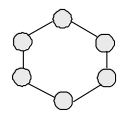
\includegraphics{./images/Blatt-1_Ring}
	\item 2. Vollständige Vermaschung: Jedes Endgäret ist mit jedem Endgerät verbunden.
	\linebreak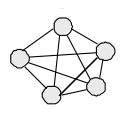
\includegraphics{./images/Blatt-1_Vollstaendige-Vermaschung}
	\item 3. Punkt-zu-Punkt Verbindung: Beide Endgeräte sind direkt miteinander verbunden.
	\linebreak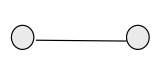
\includegraphics{./images/Blatt-1_PunktZuPunkt-Verbindung}
	\item 4. Baum: Endgeräte werden als Knoten dargestellt. Die Blätter eines Knotens sind die verbundenen Endgeräte zu dem jeweiligen Knoten (Endgerät).
	\linebreak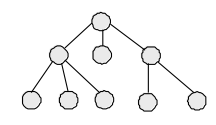
\includegraphics{./images/Blatt-1_Baum}
	\item 5. Irreguläre Vermaschung: keine klare Struktur der Verbindungen zwischen den Endgeräten.
	\linebreak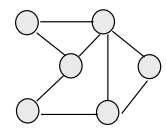
\includegraphics{./images/Blatt-1_Irregulaere-Vermanschung}
	\item 6. Bus: Alle Endgeräte können mit den anderen Endgeräten über eine gemeinsame Verbindung kommunizieren.
	\linebreak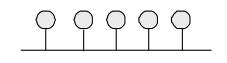
\includegraphics{./images/Blatt-1_Bus}
\end{itemize}

\subsection{b)}
\begin{itemize}
	\item Ethernet: Baum, Stern, Punkt-zu-Punkt
	\item WLAN: Stern, Broadcast
	\item Satellitennetze: Vermaschung, Broadcast
\end{itemize}

\subsection{c)}
Bei einer physischen Topologie müssen wir die Verkabelung konkreter Hardware betrachten.
Zum Beispiel Kabel, Switches, Radiokarten oder Antennen. Die logische
Topologie wird von dem Kommunikationsmodell der Software bestimmt.

\subsection{d)}
\begin{itemize}
	\item physikalischer Stern mit logischem Stern: Fileserver in einem
	kleinen Firmennetzwerk (Anwendungsschicht)
	\item physikalischer Stern mit logischem Ring: Token-Ring - sternvörmige Verkabelung der Endgeräte mit einem Verteiler. Dieser Verteiler sendet ein Token an das nächst liegende Endgerät im logischen Ring.
	\item physikalischer Bus mit logischem Ring:  Profibus - Master und Slaves liegen auf dem selben Bus, allerdings kommunizieren die Master jeweils nur mit den anderen Master in einem logischen Ring. Ebenso wie die Slaves. (Netzzugangsschicht)
	\item physiaklische irreguläre Vermaschung mit logischer Punkt-zu-Punkt Verbindung: Torrent über Internet (Anwendungsschicht)	
\end{itemize}

\subsection{e)}
\begin{itemize}
	\item Stern (WLAN) + Punkt-zu-Punkt (Webserver zu AP) (logisch: TCP/IP Punkt-zu-Punkt)
	\item Stern (WLAN) + Punkt-zu-Punkt (Switch zu AP) + Baum (Switch zu Webserver) (logisch: TCP/IP Punkt-zu-Punkt)
	\item Punkt-zu-Punkt (WLAN) + Stern (Konferenzserver) (logisch: TCP/IP Punkt-zu-Punkt)
\end{itemize}

\section{Aufgabe 4}
\subsection{a)}
Ein Protokoll hat die Aufgabe, den beteiligten Kommunikationspartnern eine
effiziente und fehlerrobuste Kommunikation zu ermöglichen. Alle Partner müssen
auf exakt dieselbe Weise kommunizieren.
Eine verteilte Diensterbringung ist ohne ein geeignetes Protokoll daher nicht möglich, da so beide Partner keine gemeinsamen Regeln für die Kommunikation besäßen.

\subsection{b)}
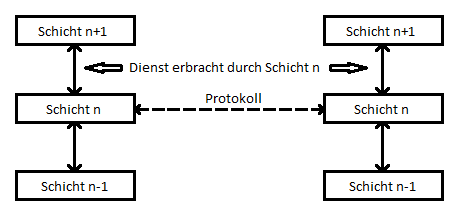
\includegraphics{./images/Blatt-1_Aufgabe4b}
\subsection{c)}
\subsubsection{i)}
Ein Dienst ist in der Regel protokollunabhängig und kann sogar gleichzeitig
mehrere Protokolle verwenden.

\subsubsection{ii)}
Es können mehrere Dienste mithilfe eines Protokolls erbracht werden, wenn zum Beispiel die Daten die übertragen werden gleich sind
aber sie vom jeweiligen Dienst zu einem anderen zweck verwendet werden.

\subsubsection{iii)}
Es können mehrere Dienstschnittstellen bereitgestellt werden. Man könnte im Protokoll zum Beispiel einen Integer übergeben der entscheidet mit welcher Dienstschnitstelle er kommunizieren möchte.

\subsection{d)}
Nachteile:
\begin{itemize}
	\item Mehr Verzögerung
\end{itemize}
Vorteile:
\begin{itemize}
	\item Mehr Abstraktion und Ausfallsicherheit
	\item leichter zu testen (jede Schicht einzelnd testen)
	\item  bessere Standardisierungsmöglichkeiten (jede Schicht enthällt eigene Protokolle)
	\item Komplexität wird verringert, dadurch das jede Schicht nur die Daten erhällt die sie benötigt
\end{itemize}

\subsection{e)}

\section{Aufgabe 5}
\subsection{a)}
Kommunikationspartner können nur dann miteinander reden, wenn sie dasselbe
Protokoll benutzen. Wenn sich jeder ein eigenes Protokoll ausdenkt, hilft
auch die beste physikalische Topologie nicht, wenn niemand die Pakete des
anderen interpretieren kann.

\subsection{b)}
Ein De-facto-Standard ist ein Industriestandard, der meistens organisch
entwickelt wurde und nicht von einem Komitee verabschiedet wurden.
Ein De-jure-Standard ist ein designter Standard, der von einem Komitee
entwickelt wurde.

\subsection{c)}
\begin{itemize}
	\item 3GPP: Third Generation Partnership Project (Mobilfunk)
	\item IEEE: Institute of Electrical and Electronics Engineers (Techniken, Hardware und Software)
	\item IETF: Internet Engineering Task Force (Internet)
	\item ISO: International Organisation for Standardization (allgemeine Standardisierung)
	\item ITU-T: International Telecommunication Union (Telekommunikation)
	\item NIST: National Insitute of Standards and Technology (allgemeine Technologiestandards)
	\item W3C: World Wide Web Consortium (Web-Standards)
\end{itemize}

\end{document}
